\chapter{10 Questions with a Millionaire: Robert Miller on Cash Flow, Scarcity, and Compounding Skill}

This chapter unfolds in the same order as the interview itself. We are first shown the payoff, namely that a personal brand can survive failed companies and accelerate later launches, and only afterward are we walked back through the machinery: school, early crypto gains, the search for cash flow, the scaling sequence of marketing, sales, and finance, the move from tactics to frameworks, the geometry of partnership, the strange question of value in crypto, and finally the difference between borrowing to patch fragility and investing to enlarge capability. There is no board mathematics here, but there is a real quantitative spine, and it helps to write that spine down with care.

\begin{remark}
The displayed formulas in this chapter are transcript-driven reconstructions. They do not come from a visible board. Their purpose is to preserve the logic of the lecture in a compact form: capital gains versus cash flow, traffic-to-revenue scaling, the rough partner bound, the scarcity-and-energy analogy, and the update rule by which self-investment compounds into later traction.
\end{remark}

\section{Prologue and Reset}

The interview does not begin at the beginning. It begins with a consequence. Robert says that while building his first agency he was also building a personal brand; that company closed, the next one closed as well, and yet the later business scaled to multiple seven figures in roughly six months because the brand had survived the shutdown of the earlier operating vehicles. He adds that a still later business reached a seven-figure runway in about sixty days.

We should keep the structure of that opening intact. The lecture is not yet explaining anything; it is showing us the end of a chain and asking us, implicitly, how such a thing is possible. Only then do we get the formal reset: the interviewer introduces the series, introduces Robert Miller as entrepreneur, investor, and multimillionaire, and asks for a quick account of his background.

That reset matters because it establishes the pattern for the whole lecture. We are not given a thesis and then a list of supporting bullets. We are given a result, then a rewind, then a stepwise reconstruction. The chapter should therefore move with the same rhythm: from durable reputation, back to origin, and then forward again through the mechanisms that make the opening claim credible.

\section{From School to Cash Flow}

Robert's background begins in digital marketing, e-commerce, and crypto, with the last of these reaching back to high school. The first real turn, however, comes when the interviewer asks what happened after high school and whether college is necessary. Robert answers in a narrower way than the slogan version of this debate would allow. He did go to college, studying business administration and economics, but the school system did not fit the path he was actually trying to identify. The decisive move came from outside the university, through a digital-marketing course.

At the same time, he had already made money in crypto. The important point is that he refuses to confuse this with the thing he later wanted to build. He says it directly: that money was capital gains, not cash flow. We should keep the distinction explicit:
\begin{align}
CG &\neq CF,\\
\Delta W &= CG + CF.
\end{align}
Here \(CG\) denotes capital gains and \(CF\) denotes cash flow. The second line is merely bookkeeping, but the lecture's real emphasis is strategic. A person may have an increase in wealth without yet possessing a business that generates recurring inflow.

Once this distinction is made, the rest of the section follows cleanly. The problem is no longer ``How do I make money once?'' but rather ``How do I build a real business?'' This is why Robert's answer about college is so tightly framed. For professions requiring formal pedigree, credentials remain necessary. But for entrepreneurship the operative requirement is different: one must solve problems and construct a mechanism that produces cash flow. The narrative hinge is not school against no school; it is passive appreciation against operating structure.

\section{Scaling as a Three-Stage Pipeline}

Once the lecture has moved from biography to practice, Robert gives the first genuinely compact model in the interview. If we want to scale a business, he says, we must master marketing and bring in more revenue. But here ``marketing'' does not reduce to buying ads. He emphasizes content, traffic strategy, and the harder question of getting people to care. From there we move to sales, because attention that never converts remains inert. Finally we arrive at finance, because even after revenue appears, someone still has to understand how the cash flows work.

\begin{figure}[h]
\centering
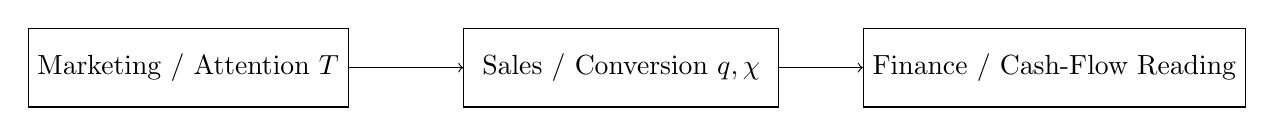
\begin{tikzpicture}
\node[draw, rectangle, minimum width=4cm, minimum height=1cm] (m) at (0,0) {Marketing / Attention \(T\)};
\node[draw, rectangle, minimum width=4cm, minimum height=1cm] (s) at (5.5,0) {Sales / Conversion \(q,\chi\)};
\node[draw, rectangle, minimum width=4cm, minimum height=1cm] (f) at (11,0) {Finance / Cash-Flow Reading};
\draw[->] (m) -- (s);
\draw[->] (s) -- (f);
\end{tikzpicture}
\caption{An editorial diagram of the sequence stated in the interview: first generate attention, then convert it, then understand the resulting cash structure.}
\end{figure}

A concise symbolic compression is
\begin{equation}
R \propto T \times q \times \chi,
\end{equation}
where \(R\) is revenue, \(T\) is traffic or attention, \(q\) is conversion from attention into genuine opportunity, and \(\chi\) is sales effectiveness. Robert does not write this formula, and we should not pretend that he does. But it faithfully captures the order in which he names the levers.

If we compare one period to the next, we get a useful growth heuristic:
\begin{equation}
\frac{R_{t+1}}{R_t}
\approx
\frac{T_{t+1}}{T_t}
\cdot
\frac{q_{t+1}}{q_t}
\cdot
\frac{\chi_{t+1}}{\chi_t}.
\end{equation}
The lecture's point is not that business obeys a literal law of motion of this form. The point is more modest and more useful: growth usually comes from improvements at several linked stages, not from a single tactical obsession.

And now we can see why finance arrives third rather than first. It is not secondary. It is interpretive. It reads the consequences of the first two stages. High revenue does not yet mean clean business control. Revenue can appear before payout timing, cash position, and risk structure are understood. The finance step is the place where the story stops being exciting and starts becoming intelligible.

\section{Books, Brand, and Partnership Structure}

The interviewer next asks for the top three books everyone should read. Robert answers in the same order in which he has just built the business problem: first strategy, then people, then revenue systems.

\begin{itemize}
\item \emph{The Road Less Stupid} is recommended as a source of mental frameworks: how to think ahead, how to think about what one is doing, and how to stop living entirely at the tactical level.
\item \emph{Multipliers} is recommended for team construction: how to work with other people, multiply their effort, and align interests.
\item \emph{Predictable Revenue} is recommended as a sales-system book: how revenue is brought in through an organized team rather than by sporadic heroics.
\end{itemize}

\subsection{Question \& Answer}

\paragraph{Question.}
What does it mean, in this lecture, to move from tactics to frameworks?

\paragraph{Answer.}
It means that we stop being satisfied with being merely the expert, the marketer, or the tactical operator. A framework asks what must be thought about before the obvious problem arrives. It asks how an offer will be rolled out, who is accountable, how a team is held to a structure, and how one sees the business from above rather than only from within. That is why the first book matters so much in Robert's account: it changes the level at which one is thinking.

From books the lecture pivots naturally to personal brand, because once strategy is on the table, durability becomes the next question. Robert says that personal brand matters because the mechanism of what one does for people changes as the market changes. Businesses do not typically last forever. Offers change. Acquisition channels change. Yet the personal brand can persist when a particular mechanism disappears. This returns us to the prologue and now explains it from the inside.

At this point the interviewer shifts to failure. Robert responds first with a practical bound:
\begin{equation}
N_p \lesssim 3,
\end{equation}
where \(N_p\) denotes the number of partners. This is not a theorem, but it is very much a rule of thumb stated with conviction: one does not need four or five partners in a company.

The lecture then elaborates the geometry behind that rule. A partner must bring something crucial to the business---connections, people, capital, execution, network---rather than merely being someone one likes. Values must align. Vision must align. And one must be willing to have a real conversation: where are we going, what are you bringing to the table, what am I bringing, and how will we call one another out when performance slips.

There is also a deeper demotion of ego here. Robert says that a name or an offer means little unless it is executed. That claim matters because it ties the failure section back to the earlier books section. Once we move from tactics to frameworks, the next unavoidable subject is accountability. The lecture is not content to say that teams matter; it insists that executional symmetry matters, that optimism and realism may have to balance one another, and that a company can be held captive if a partner is nominally central without being properly aligned.

\section{Cryptocurrency as a Question About Value}

When the interviewer asks about crypto, the lecture widens abruptly. We are no longer only in the world of business technique. Robert presents crypto not merely as a profitable niche or a new technology, but as a new way of thinking about money. He immediately expands the frame beyond Bitcoin and Ethereum alone and brings in central banks, CBDCs, the question of where wealth should be stored, and the deeper issue of what society counts as valuable.

This section should be handled carefully. Robert is not presenting a finished theory of money. He is staging a conceptual difficulty and thinking aloud through an analogy.

\subsection{Question \& Answer}

\paragraph{Question.}
Is value grounded in rarity alone, or in scarcity backed by real cost?

\paragraph{Answer.}
Robert raises the contrast explicitly. Perhaps an asset is valuable simply because it is rare. But perhaps value becomes more persuasive when real physical cost is tied to its creation or verification. Bitcoin enters through mining and the electricity required to verify transactions. Gold enters through extraction and mining cost. The interview does not prove a theorem; it offers a way to think.

A cautious symbolic compression is
\begin{equation}
V_{\text{asset}} \propto \sigma \, E_{\text{cost}},
\end{equation}
where \(\sigma\) is scarcity and \(E_{\text{cost}}\) is real extraction or verification cost. This formula is editorial, not spoken, and it should be read only as a memory device for the analogy.

The logic of the section can be written in a short derivation:
\begin{enumerate}
\item Ask whether value is merely rarity.
\item Ask whether value requires real cost as well.
\item Introduce Bitcoin as an asset whose verification requires physical electricity and mining infrastructure.
\item Introduce gold as an asset whose extraction requires mining and energy.
\item Infer that society may distinguish between costless rarity and energy-backed scarcity.
\item Leave open the practical question: do we transact with such an asset, or do we preserve wealth in it?
\end{enumerate}

The lecture deliberately refuses to close the question too quickly. Robert asks what Web3.0 will look like and what a CBDC rollout will look like. He also utters a garbled phrase in the transcript about changing how we operate, so it is safer to keep the final issue broad: crypto may alter how value, surveillance, and wealth storage are jointly imagined, but the interview stops short of doctrinal precision.

\section{From First Break to Compounding Skill}

Once the abstract question of value has been raised, the interviewer brings the lecture back down to biography by asking what got Robert into crypto in the first place. This transition matters. The lecture does not want theory floating free of experience; it wants the conceptual section to be anchored in a concrete path.

Robert places the beginning around 2015--2016. He and his brother met someone who was deeply immersed in that world, and through repeated conversations they encountered the idea of Bitcoin at an unusually early stage. He reports wallet figures and transaction magnitudes that are impossible to verify from the interview alone, so the proper attitude here is simply to preserve them as his report and not sharpen them into audited fact. What matters structurally is the sequence: curiosity, repeated exposure, early price awareness, and then participation.

He gives concrete price anchors. Bitcoin was around \$800--\$1{,}000. Ethereum was about \$17. AntShares later became Neo, and he describes that as one of the projects on which he did particularly well. The worked numerical example in the lecture is striking enough that it should be preserved in compact form:
\begin{align}
I_0 &\approx (1.5\text{--}2.0)\times 10^3 \text{ dollars},\\
V_{4m} &\approx 2.5\times 10^5 \text{ dollars},\\
M &= \frac{V_{4m}}{I_0} \approx 125\text{--}167.
\end{align}
This is not a valuation model; it is a scale-preserving summary of the anecdote. The interview's emotional force here lies in the disproportion: a small stake expands into something life-changing within a short period. Robert then says that the result was not merely excitement. It produced a desire to explain the phenomenon to other people. He began creating books and courses, giving them away for free, and speaking on stages. Teaching, in this account, becomes an early form of entrepreneurship.

The interviewer then asks whether this was his first big financial break, and Robert answers yes. That answer matters because it sets up the next pair of questions, which are among the sharpest in the lecture: the worst financial decision and the best financial decision.

The worst decision is not a speculative bet gone bad. It is an organizationally revealing financing episode. A payment-processing problem created a cash crunch. Robert says he took out what he calls a flash loan to cover payroll. The transcript does not allow us to determine whether this is the precise technical sense of the term or a looser description of short-term borrowing, so we should remain cautious. But the structure is clear: the borrowing was used to patch an immediate operational gap.

What made the decision bad, in his telling, was not only the existence of debt. It was the asymmetry. He took the risk to keep the company moving, and the others did not meaningfully share it. The borrowing therefore exposed the partnership structure rather than merely the balance sheet. In the lecture's own logic, the financial mistake is diagnostic.

\subsection{Question \& Answer}

\paragraph{Question.}
What distinguishes destructive leverage from compounding self-investment?

\paragraph{Answer.}
In the interview, destructive leverage is borrowing against fragility in order to keep a weak structure alive for one more cycle. Compounding self-investment is the opposite: it purchases frameworks, skills, and exposure that increase later earning power. The payroll borrowing revealed asymmetry and weak commitment. The course and mentorship spending, by contrast, raised Robert's capability and later traction.

That contrast becomes explicit in the next answer. After the crypto gains, Robert says that he put roughly \$30{,}000--\$40{,}000 into courses, learning stocks, e-commerce, and marketing. He is careful here: he does not claim that one should become an expert in everything. He says instead that one should become versatile enough to understand several domains while still remaining primarily committed to one.

The lecture's compounding logic can be written as an update rule:
\begin{align}
K_{t+1} &= K_t + \Delta K(I_t),\\
R_{t+1} &= R\bigl(K_{t+1}\bigr),
\end{align}
where \(K_t\) is accumulated capability and \(I_t\) is investment in courses, mentorships, or high-exposure environments. Again, this is an editorial formalization, not a quoted formula. But it captures the lecture's causal claim: skill compounds, and later revenue is downstream of that accumulation.

Robert makes one further refinement that is worth preserving. Sometimes the last mastermind or the last mentorship looks like the catalyst that changed everything. But, in his telling, that catalyst works only because earlier layers were already in place. This is a subtle point. The lecture is not describing a one-shot conversion experience. It is describing stacked preparation. Exposure compounds. Frameworks compound. Judgment compounds. Then, at some later point, the visible revenue jump appears.

\section{Relationships, Health, and the Evolving Why}

The lecture now widens again, and it is important not to treat this as mere inspirational tail matter. The interviewer asks for the greatest lesson Robert has learned so far. His answer is about relationships, but not in a vague social sense. The right relationships matter the most. He asks us to imagine a situation in which we have only three numbers to dial. Who, then, is really there? The lecture's commercial logic is widening into a deeper test of structure and loyalty.

From there Robert moves to health. He describes an extreme period of overwork in which he was balancing full-time work and school, running on almost no sleep, and eventually had a frightening physical episode at home. The details are less important than the function of the anecdote. Up to this point the chapter has been about traffic, sales, finance, brand, partnership, value, and education. Now the lecture reintroduces the body as a constraint. The real ledger contains more than revenue and asset prices.

The final question asks for his long-term goal and what motivates him to keep going. Robert begins by reorganizing the answer: let us start with the why first. That reframing is itself a signal. The order matters. He first recalls a childhood marked by financial insecurity and hunger, and the initial motivation is therefore simple: never let his family experience that kind of lack again. But he then says that the why evolves. Once the basic needs are met, the aim is no longer merely food or immediate security. It becomes the chase after potential, impact, greater personal capability, and the power to care for one's family from a position of strength.

This final section is where the whole lecture coheres. Money is not rejected. It is repositioned. It becomes the instrument through which several deeper commitments are made operative: the protection of family, the cultivation of health, the honoring of relationships, and the pursuit of a more developed self. That is why the lecture ends where it does. The business story is real, but it is nested inside a larger human order.

\section{Summary}

The interview begins with a bold effect and then patiently reconstructs the machinery behind it. Personal brand survives the collapse of particular operating vehicles; capital gains are not the same as cash flow; scaling requires marketing, sales, and finance in sequence; books matter because they move us from tactics to frameworks; partnership fails when execution, contribution, and values are not aligned; crypto becomes interesting when it raises the question of scarcity and cost; and financial judgment becomes mature when windfalls are turned into durable capability rather than mistaken for a finished identity.

The last movement of the lecture is the most important one. Relationships, health, and family are not appendices to the business story. They are the frame within which that story becomes legible at all. What begins as a conversation about money ends as a conversation about what money is finally for.